%%%%%%%%%%%%%%%%%%%%%%%%%%%%%%%%%%%%%%%%%
% BA04 presentation 
% LaTeX Template
% Version 1.0 (14/12/14)
%
% This template has been downloaded from:
% http://www.LaTeXTemplates.com
%
% License:
% CC BY-NC-SA 3.0 (http://creativecommons.org/licenses/by-nc-sa/3.0/)
%
%%%%%%%%%%%%%%%%%%%%%%%%a%%%%%%%%%%%%%%%%%

%----------------------------------------------------------------------------------------
%	PACKAGES AND THEMES
%----------------------------------------------------------------------------------------

\documentclass[9pt]{beamer}

\mode<presentation> {

% The Beamer class comes with a number of default slide themes
% which change the colors and layouts of slides. Below this is a list
% of all the themes, uncomment each in turn to see what they look like.

%\usetheme{default}
%\usetheme{AnnArbor}
%\usetheme{Antibes}
%\usetheme{Bergen}
%\usetheme{Berkeley}
%\usetheme{Berlin}
%\usetheme{Boadilla}
%\usetheme{CambridgeUS}
%\usetheme{Copenhagen}
%\usetheme{Darmstadt}
%\usetheme{Dresden}
%\usetheme{Frankfurt}
%\usetheme{Goettingen}
%\usetheme{Hannover}
%\usetheme{Ilmenau}
%\usetheme{JuanLesPins}
%\usetheme{Luebeck}
\usetheme{Madrid}
%\usetheme{Malmoe}
%\usetheme{Marburg}
%\usetheme{Montpellier}
%\usetheme{PaloAlto}
%\usetheme{Pittsburgh}
%\usetheme{Rochester}
%\usetheme{Singapore}
%\usetheme{Szeged}
%\usetheme{Warsaw}

% As well as themes, the Beamer class has a number of color themes
% for any slide theme. Uncomment each of these in turn to see how it
% changes the colors of your current slide theme.

%\usecolortheme{albatross}
\usecolortheme{beaver}
%\usecolortheme{beetle}
%\usecolortheme{crane}
%\usecolortheme{dolphin}
%\usecolortheme{dove}
%\usecolortheme{fly}
%\usecolortheme{lily}
%\usecolortheme{orchid}
%\usecolortheme{rose}
%\usecolortheme{seagull}
%\usecolortheme{seahorse}
%\usecolortheme{whale}
%\usecolortheme{wolverine}

%\setbeamertemplate{footline} % To remove the footer line in all slides uncomment this line
%\setbeamertemplate{footline}[page number] % To replace the footer line in all slides with a simple slide count uncomment this line

\setbeamertemplate{navigation symbols}{} % To remove the navigation symbols from the bottom of all slides uncomment this line
\setbeamerfont{frametitle}{size=\normalsize}
}

\usepackage{graphicx} % Allows including images
\usepackage{booktabs} % Allows the use of \toprule, \midrule and \bottomrule in tables
\usepackage[english]{babel}
\usepackage[utf8x]{inputenc}
\usepackage{hyperref}
%\usepackage{underscore}


\graphicspath{
				{../weights/}
			 }

\newcommand{\backupbegin}{
	\newcounter{finalframe}
	\setcounter{finalframe}{\value{framenumber}}
}
\newcommand{\backupend}{
	\setcounter{framenumber}{\value{finalframe}}
}

\begin{document}
%----------------------------------------------------------------------------------------\\
%----------------------------------------------------------------------------------------\\
%\begin{frame}
%	\frametitle{Horizontal template morphing}
%	\textbf{Reminder}\\
%	\vspace{0.2cm}
%	Shape comes from CDF shift between $cdf_{Z peak}^{0b}$ and $cdf_{Z peak}^{1b/2b}$\\
%	\vspace{0.1cm}
%	Shift applied to $cdf_{Z veto}^{0b} \rightarrow cdf_{Z veto}^{1b/2b} \rightarrow cdf_{Z veto}^{1b/2b}(norm) $\\
%	\vspace{0.1cm}
%	Numerical factor : $N_{Z veto}^{0b}(corr) \times \frac{N_{Z peak}^{1b/2b}}{N_{Z peak}^{0b}}$ 
%	\begin{itemize}
%		\item $N_{Z veto}^{0b}(corr)$ 
%		\begin{itemize}
%			\item data : correction factor from combine fit in SR 0b
%			\item MC : 1.0 (by closure definition)
%		\end{itemize}
%		\item $N_{Z peak}^{1b/2b}$ and $N_{Z peak}^{0b}$
%		\begin{itemize}
%			\item data : correction factor from combine fit in SR 1b and 2b
%			\item MC : DY MC histogram integral
%		\end{itemize}
%	\end{itemize}
%	In next slides, results will be for the closure (aka the MC bullet)\\
%	Note : using the DNN with the btag discriminant information
%\end{frame}
%********************************************************************************************************
%********************************************************************************************************
%********************************************************************************************************
\begin{frame}
	\frametitle{DY DNN Output : SSDL channel}
	\hspace{2.0cm} \textbf{DNN 01} \hspace{4cm} \textbf{DNN 02} 
	\begin{figure}
		\includegraphics[page=4,width=0.45\linewidth]{weight_DNNoutputDY_SSDL_mc_DNN01_1D_CDFShift1b.pdf}
		\includegraphics[page=4,width=0.45\linewidth]{weight_DNNoutputDY_SSDL_mc_DNN02_1D_CDFShift1b.pdf}\\
		\includegraphics[page=4,width=0.45\linewidth]{weight_DNNoutputDY_SSDL_mc_DNN01_1D_CDFShift2b.pdf}
		\includegraphics[page=4,width=0.45\linewidth]{weight_DNNoutputDY_SSDL_mc_DNN02_1D_CDFShift2b.pdf}
	\end{figure}
\end{frame}
%********************************************************************************************************
\begin{frame}
	\frametitle{TT DNN Output : SSDL channel}
	\hspace{2.0cm} \textbf{DNN 01} \hspace{4cm} \textbf{DNN 02} 
	\begin{figure}
		\includegraphics[page=4,width=0.45\linewidth]{weight_DNNoutputTT_SSDL_mc_DNN01_1D_CDFShift1b.pdf}
		\includegraphics[page=4,width=0.45\linewidth]{weight_DNNoutputTT_SSDL_mc_DNN02_1D_CDFShift1b.pdf}\\
		\includegraphics[page=4,width=0.45\linewidth]{weight_DNNoutputTT_SSDL_mc_DNN01_1D_CDFShift2b.pdf}
		\includegraphics[page=4,width=0.45\linewidth]{weight_DNNoutputTT_SSDL_mc_DNN02_1D_CDFShift2b.pdf}
	\end{figure}
\end{frame}
%********************************************************************************************************
\begin{frame}
	\frametitle{ST DNN Output : SSDL channel}
	\hspace{2.0cm} \textbf{DNN 01} \hspace{4cm} \textbf{DNN 02} 
	\begin{figure}
		\includegraphics[page=4,width=0.45\linewidth]{weight_DNNoutputST_SSDL_mc_DNN01_1D_CDFShift1b.pdf}
		\includegraphics[page=4,width=0.45\linewidth]{weight_DNNoutputST_SSDL_mc_DNN02_1D_CDFShift1b.pdf}\\
		\includegraphics[page=4,width=0.45\linewidth]{weight_DNNoutputST_SSDL_mc_DNN01_1D_CDFShift2b.pdf}
		\includegraphics[page=4,width=0.45\linewidth]{weight_DNNoutputST_SSDL_mc_DNN02_1D_CDFShift2b.pdf}
	\end{figure}
\end{frame}
%********************************************************************************************************
\begin{frame}
	\frametitle{TTVX DNN Output : SSDL channel}
	\hspace{2.0cm} \textbf{DNN 01} \hspace{4cm} \textbf{DNN 02} 
	\begin{figure}
		\includegraphics[page=4,width=0.45\linewidth]{weight_DNNoutputTTVX_SSDL_mc_DNN01_1D_CDFShift1b.pdf}
		\includegraphics[page=4,width=0.45\linewidth]{weight_DNNoutputTTVX_SSDL_mc_DNN02_1D_CDFShift1b.pdf}\\
		\includegraphics[page=4,width=0.45\linewidth]{weight_DNNoutputTTVX_SSDL_mc_DNN01_1D_CDFShift2b.pdf}
		\includegraphics[page=4,width=0.45\linewidth]{weight_DNNoutputTTVX_SSDL_mc_DNN02_1D_CDFShift2b.pdf}
	\end{figure}
\end{frame}
%********************************************************************************************************
\begin{frame}
	\frametitle{VVV DNN Output : SSDL channel}
	\hspace{2.0cm} \textbf{DNN 01} \hspace{4cm} \textbf{DNN 02} 
	\begin{figure}
		\includegraphics[page=4,width=0.45\linewidth]{weight_DNNoutputVVV_SSDL_mc_DNN01_1D_CDFShift1b.pdf}
		\includegraphics[page=4,width=0.45\linewidth]{weight_DNNoutputVVV_SSDL_mc_DNN02_1D_CDFShift1b.pdf}\\
		\includegraphics[page=4,width=0.45\linewidth]{weight_DNNoutputVVV_SSDL_mc_DNN01_1D_CDFShift2b.pdf}
		\includegraphics[page=4,width=0.45\linewidth]{weight_DNNoutputVVV_SSDL_mc_DNN02_1D_CDFShift2b.pdf}
	\end{figure}
\end{frame}
%********************************************************************************************************
\begin{frame}
	\frametitle{H DNN Output : SSDL channel}
	\hspace{2.0cm} \textbf{DNN 01} \hspace{4cm} \textbf{DNN 02} 
	\begin{figure}
		\includegraphics[page=4,width=0.45\linewidth]{weight_DNNoutputH_SSDL_mc_DNN01_1D_CDFShift1b.pdf}
		\includegraphics[page=4,width=0.45\linewidth]{weight_DNNoutputH_SSDL_mc_DNN02_1D_CDFShift1b.pdf}\\
		\includegraphics[page=4,width=0.45\linewidth]{weight_DNNoutputH_SSDL_mc_DNN01_1D_CDFShift2b.pdf}
		\includegraphics[page=4,width=0.45\linewidth]{weight_DNNoutputH_SSDL_mc_DNN02_1D_CDFShift2b.pdf}
	\end{figure}
\end{frame}
%********************************************************************************************************
\begin{frame}
	\frametitle{Rare DNN Output : SSDL channel}
	\hspace{2.0cm} \textbf{DNN 01} \hspace{4cm} \textbf{DNN 02} 
	\begin{figure}
		\includegraphics[page=4,width=0.45\linewidth]{weight_DNNoutputRare_SSDL_mc_DNN01_1D_CDFShift1b.pdf}
		\includegraphics[page=4,width=0.45\linewidth]{weight_DNNoutputRare_SSDL_mc_DNN02_1D_CDFShift1b.pdf}\\
		\includegraphics[page=4,width=0.45\linewidth]{weight_DNNoutputRare_SSDL_mc_DNN01_1D_CDFShift2b.pdf}
		\includegraphics[page=4,width=0.45\linewidth]{weight_DNNoutputRare_SSDL_mc_DNN02_1D_CDFShift2b.pdf}
	\end{figure}
\end{frame}
%********************************************************************************************************
\begin{frame}
	\frametitle{HH DNN Output : SSDL channel}
	\hspace{2.0cm} \textbf{DNN 01} \hspace{4cm} \textbf{DNN 02} 
	\begin{figure}
		\includegraphics[page=4,width=0.45\linewidth]{weight_DNNoutputHH_SSDL_mc_DNN01_1D_CDFShift1b.pdf}
		\includegraphics[page=4,width=0.45\linewidth]{weight_DNNoutputHH_SSDL_mc_DNN02_1D_CDFShift1b.pdf}\\
		\includegraphics[page=4,width=0.45\linewidth]{weight_DNNoutputHH_SSDL_mc_DNN01_1D_CDFShift2b.pdf}
		\includegraphics[page=4,width=0.45\linewidth]{weight_DNNoutputHH_SSDL_mc_DNN02_1D_CDFShift2b.pdf}
	\end{figure}
\end{frame}


\end{document}
